\PassOptionsToPackage{table}{xcolor}
\documentclass[aspectratio=169, 11pt]{beamer}

\usepackage[T1]{fontenc}
\usepackage[utf8]{inputenc}
\usepackage{lmodern}
\usepackage{microtype}
\usepackage{tikz}
\usepackage{booktabs}
\usepackage{tabularx}
\usepackage{array}
\usepackage{xcolor}
\usepackage{mdframed}
\usepackage{graphicx}

\usetikzlibrary{
  arrows.meta, positioning, shapes.geometric, shapes.misc,
  fit, backgrounds, calc, shadows
}

% ── Colour palette — MeshWhisper brand (teal) ────────────────────────────────
\definecolor{mwblue}{HTML}{014451}    % brand 900 — deep teal (title pages, frame headers)
\definecolor{mwaccent}{HTML}{0694A2}  % brand 500 — primary accent
\definecolor{mwbright}{HTML}{16BDCA}  % brand 400 — bright highlight
\definecolor{mwlight}{HTML}{D5F5F6}   % brand 100 — pale background
\definecolor{mwpale}{HTML}{EDFAFA}    % brand 50  — palest background
\definecolor{mwgray}{HTML}{6B7280}
\definecolor{mwrule}{HTML}{D1D5DB}
\definecolor{mwgreen}{HTML}{0E7C5B}
\definecolor{mwred}{HTML}{C0392B}
\definecolor{mworange}{HTML}{E67E22}
\definecolor{mwpurple}{HTML}{6B4FA0}
\definecolor{nodebg}{HTML}{EDFAFA}
\definecolor{devicebg}{HTML}{F0FFF4}
\definecolor{slidebg}{HTML}{F8FAFC}

% ── Beamer theme ─────────────────────────────────────────────────────────────
\usetheme{default}
\usecolortheme{default}
\usefonttheme{professionalfonts}
\setbeamertemplate{navigation symbols}{}
\setbeamertemplate{itemize items}{\color{mwaccent}\textbullet}
\setbeamertemplate{enumerate items}{\color{mwaccent}\insertenumlabel.}

\setbeamercolor{background canvas}{bg=slidebg}
\setbeamercolor{frametitle}{fg=white, bg=mwblue}
\setbeamercolor{title}{fg=white}
\setbeamercolor{subtitle}{fg=mwlight}
\setbeamercolor{author}{fg=mwlight}
\setbeamercolor{date}{fg=mwlight}
\setbeamercolor{normal text}{fg=mwblue}
\setbeamercolor{itemize item}{fg=mwaccent}
\setbeamercolor{itemize subitem}{fg=mwgray}
\setbeamercolor{block title}{fg=white, bg=mwaccent}
\setbeamercolor{block body}{fg=mwblue, bg=mwlight}

\setbeamertemplate{frametitle}{
  \vspace{2pt}
  \begin{beamercolorbox}[wd=\paperwidth, ht=7mm, dp=2mm, leftskip=6mm]{frametitle}
    \usebeamerfont{frametitle}\insertframetitle
  \end{beamercolorbox}
}

\setbeamertemplate{footline}{
  \begin{beamercolorbox}[wd=\paperwidth, ht=4mm, dp=1.5mm, leftskip=4mm, rightskip=4mm]{normal text}
    \color{mwgray}\tiny meshwhisper.org \hfill \insertframenumber\,/\,\inserttotalframenumber
  \end{beamercolorbox}
}

\setbeamerfont{frametitle}{size=\normalsize, series=\bfseries}
\setbeamerfont{title}{size=\LARGE, series=\bfseries}
\setbeamerfont{subtitle}{size=\normalsize}

% ── Title page ────────────────────────────────────────────────────────────────
\title{MeshWhisper}
\subtitle{Messaging as Ambient Infrastructure}
\author{meshwhisper.org}
\date{April 2026}

% ─────────────────────────────────────────────────────────────────────────────
\begin{document}

% ── Title slide ───────────────────────────────────────────────────────────────
{
\setbeamercolor{background canvas}{bg=mwblue}
\begin{frame}[plain]
\vspace{8mm}
\begin{center}
  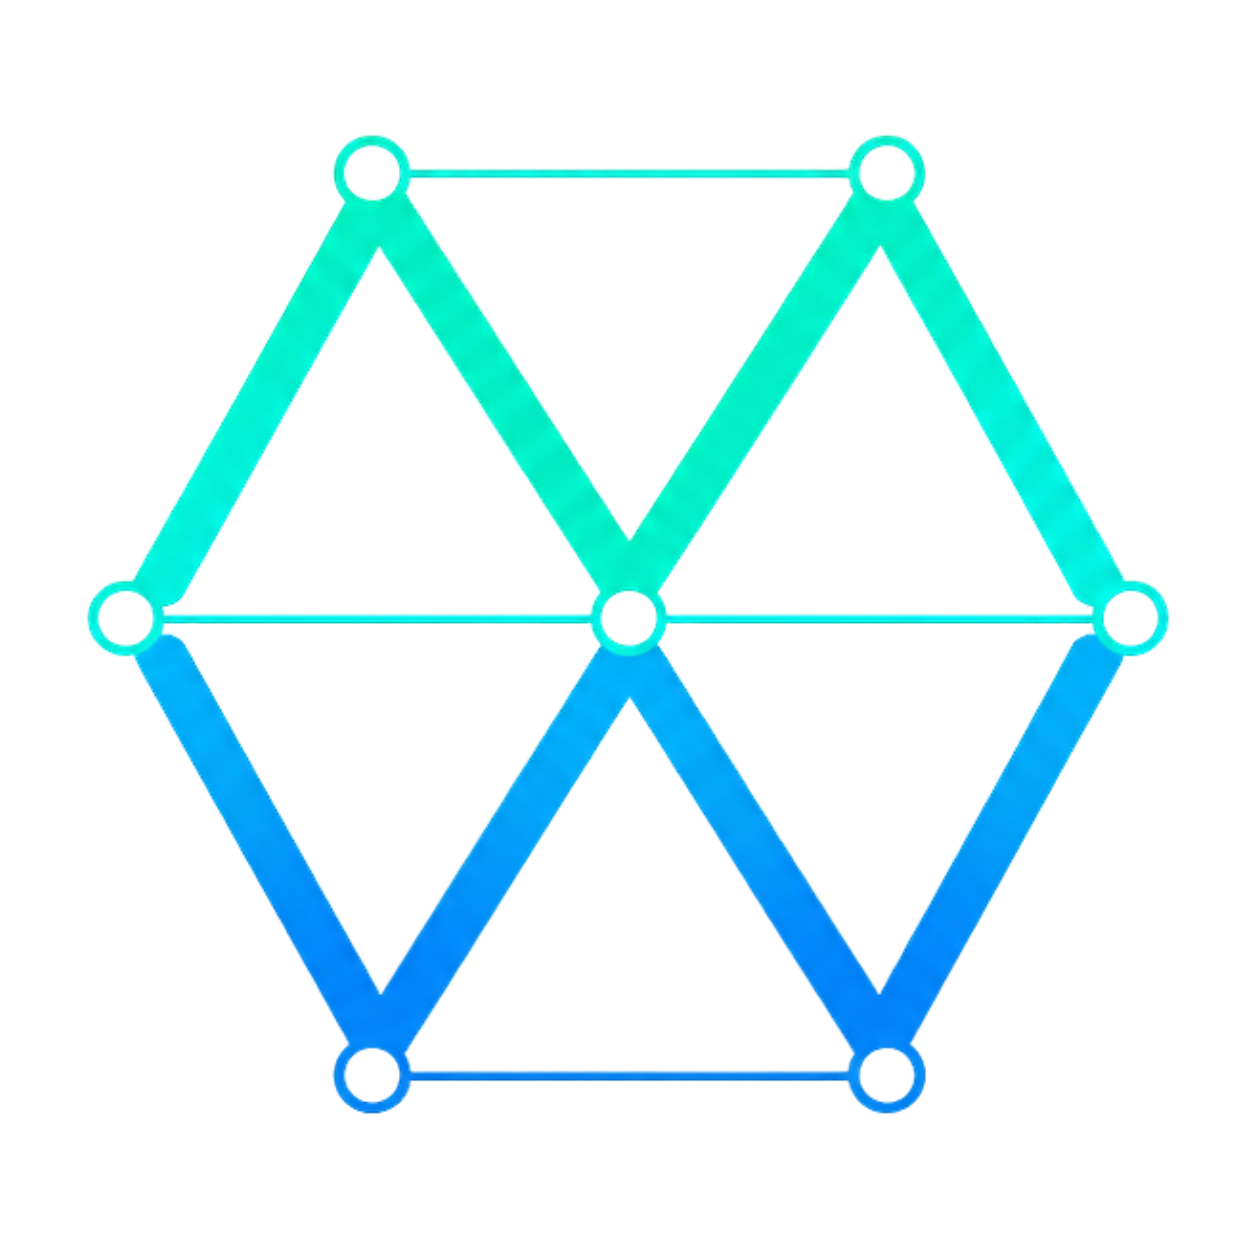
\includegraphics[width=22mm]{mw-logo-mark.png}\\[10pt]
  {\usebeamerfont{title}\color{white}MeshWhisper}\\[4pt]
  {\color{mwbright}\large Messaging as Ambient Infrastructure}\\[16pt]
  \color{mwbright}\rule{60mm}{0.4pt}\\[10pt]
  {\color{mwlight}\small meshwhisper.org · April 2026}
\end{center}
\end{frame}
}

% ── The Problem ───────────────────────────────────────────────────────────────
\begin{frame}{Every developer faces the same choice}
\vspace{2mm}
\begin{columns}[T]
  \begin{column}{0.32\textwidth}
    \begin{block}{Build it yourself}
      \small WebSocket servers, offline queuing, push notifications, media handling.
      Each piece is a project on its own.\\[4pt]
      \textbf{Cost: months of engineering}
    \end{block}
  \end{column}
  \begin{column}{0.32\textwidth}
    \begin{block}{Pay for a service}
      \small Sendbird from \$349/mo. PubNub from \$98/mo per 1k MAU.
      Costs scale aggressively.\\[4pt]
      \textbf{Cost: four figures/month at scale}
    \end{block}
  \end{column}
  \begin{column}{0.32\textwidth}
    \begin{block}{Use Firebase}
      \small Free at small scale. Every message passes through Google in readable form.
      GDPR. Vendor lock-in. Pricing cliff.\\[4pt]
      \textbf{Cost: privacy and control}
    \end{block}
  \end{column}
\end{columns}
\vspace{6mm}
\centering
\color{mwgray}\small The trilemma has a structural cause: traditional infrastructure must \emph{read} a message to route it.\\
\textbf{\color{mwblue}MeshWhisper breaks that assumption.}
\end{frame}

% ── Core Insight ──────────────────────────────────────────────────────────────
{
\setbeamercolor{background canvas}{bg=mwblue}
\begin{frame}[plain]
\vspace{18mm}
\begin{center}
  {\color{mwlight}\large\itshape ``A relay does not need to read a message to forward it.''}\\[12pt]
  \color{mwrule}\rule{80mm}{0.4pt}\\[10pt]
  {\color{mwgray}\small If messages are encrypted before they leave the device,\\
  a relay is just a pipe. It forwards an opaque blob.\\[6pt]
  The relay cannot read the content. It doesn't need to.}
\end{center}
\end{frame}
}

% ── Architecture ──────────────────────────────────────────────────────────────
\begin{frame}{Two layers, one protocol}
\begin{columns}[T]
  \begin{column}{0.48\textwidth}
    \vspace{1mm}
    {\color{mwaccent}\textbf{Node Layer — the backbone}}\\[3pt]
    \small
    Deployed by each app developer. One Docker container, one port.
    \begin{itemize}\small
      \item Packet relay and store-and-forward
      \item Push notification forwarding (APNs / FCM)
      \item Encrypted media storage
      \item Prekey directory for first contact
    \end{itemize}
    \vspace{4pt}
    Always on. Never holds a decryption key.\\
    A post box, not a postman.
    \vspace{6pt}

    {\color{mwgreen}\textbf{Device Layer — the mesh}}\\[3pt]
    \small
    Every SDK-embedded device relays for every other.
    \begin{itemize}\small
      \item Platform P2P (Multipeer / Nearby)
      \item Local network
      \item Internet (connectable peers)
    \end{itemize}
    Grows organically with adoption.
  \end{column}
  \begin{column}{0.48\textwidth}
    \vspace{2mm}
    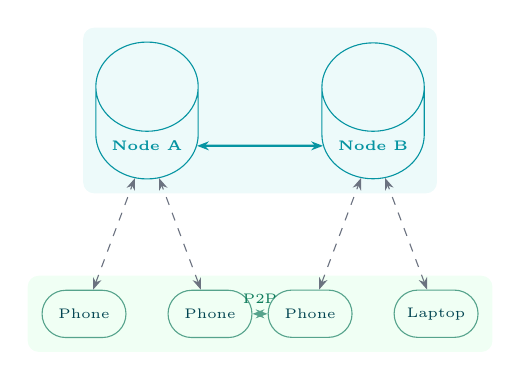
\begin{tikzpicture}[scale=0.82,
      mwnode/.style={cylinder, shape border rotate=90, draw=mwaccent,
        fill=nodebg, minimum width=13mm, minimum height=9mm,
        font=\tiny\bfseries, text=mwaccent},
      phone/.style={rounded rectangle, draw=mwgreen!70, fill=devicebg,
        minimum width=13mm, minimum height=6mm, font=\tiny, text=mwblue},
      node distance=6mm
    ]
      \node[mwnode] (n1) {Node A};
      \node[mwnode, right=16mm of n1] (n2) {Node B};
      \draw[thick, mwaccent, {Stealth[length=1.5mm]}-{Stealth[length=1.5mm]}] (n1) -- (n2);
      \node[phone, below=14mm of n1, xshift=-8mm] (p1) {Phone};
      \node[phone, below=14mm of n1, xshift=8mm]  (p2) {Phone};
      \node[phone, below=14mm of n2, xshift=-8mm] (p3) {Phone};
      \node[phone, below=14mm of n2, xshift=8mm]  (p4) {Laptop};
      \draw[mwgray, dashed, {Stealth[length=1.5mm]}-{Stealth[length=1.5mm]}] (p1) -- (n1);
      \draw[mwgray, dashed, {Stealth[length=1.5mm]}-{Stealth[length=1.5mm]}] (p2) -- (n1);
      \draw[mwgray, dashed, {Stealth[length=1.5mm]}-{Stealth[length=1.5mm]}] (p3) -- (n2);
      \draw[mwgray, dashed, {Stealth[length=1.5mm]}-{Stealth[length=1.5mm]}] (p4) -- (n2);
      \draw[mwgreen!70, thick, {Stealth[length=1.5mm]}-{Stealth[length=1.5mm]}]
        (p2) -- node[font=\tiny, text=mwgreen, above, sloped]{P2P} (p3);
      \begin{scope}[on background layer]
        \node[fill=nodebg, rounded corners=4pt, fit=(n1)(n2), inner sep=5pt] {};
        \node[fill=devicebg, rounded corners=4pt, fit=(p1)(p2)(p3)(p4), inner sep=5pt] {};
      \end{scope}
    \end{tikzpicture}
  \end{column}
\end{columns}
\end{frame}

% ── Developer Integration ─────────────────────────────────────────────────────
\begin{frame}{Integrate in an afternoon}
\vspace{2mm}
\begin{columns}[T]
  \begin{column}{0.50\textwidth}
    \begin{tabularx}{\linewidth}{@{}>{\bfseries\small}lX@{}}
    \toprule
    Step & \\
    \midrule
    Deploy  & \texttt{\small docker run meshwhisper/node} \\[3pt]
    Install & \texttt{\small npm install @meshwhisper/sdk} \\[3pt]
    Init    & \texttt{\small MeshWhisper.init(\{...\})} \\[3pt]
    Send    & \texttt{\small sendMessage(id, payload)} \\[3pt]
    Receive & \texttt{\small onMessage: msg => ...} \\
    \bottomrule
    \end{tabularx}
  \end{column}
  \begin{column}{0.46\textwidth}
    \vspace{1mm}
    \begin{tabularx}{\linewidth}{@{}XX@{}}
    \toprule
    \textbf{\small\color{mwblue}You own} & \textbf{\small\color{mwblue}MeshWhisper owns} \\
    \midrule
    \small User identity & \small Key exchange (PQXDH) \\
    \small Message content & \small Session encryption \\
    \small Your Node & \small Routing \& relay \\
    \small Your users' data & \small Store-and-forward \\
    \small Your UI & \small Push dispatch \\
    \bottomrule
    \end{tabularx}
  \end{column}
\end{columns}
\vspace{5mm}
\centering
{\small\color{mwgray}Post-quantum E2EE with zero cryptographic decisions required.}
\end{frame}

% ── Namespace Isolation ───────────────────────────────────────────────────────
\begin{frame}{Namespace isolation — cryptographic, not configured}
\vspace{3mm}
\begin{center}
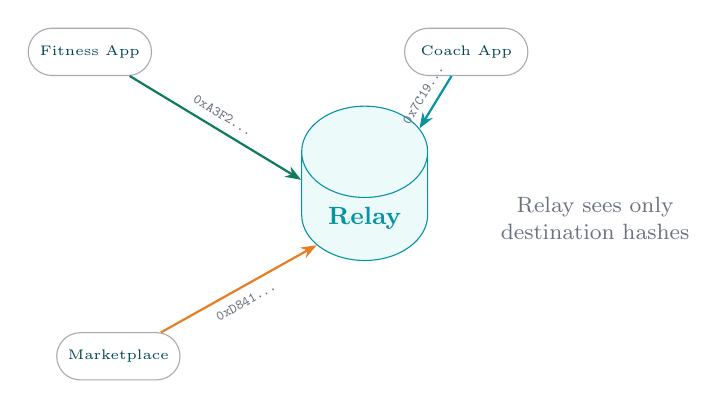
\begin{tikzpicture}[scale=0.9,
  blob/.style={rounded rectangle, draw=mwgray!60, fill=white,
    minimum width=18mm, minimum height=6mm, font=\tiny, text=mwblue},
  relay/.style={cylinder, shape border rotate=90, draw=mwaccent,
    fill=nodebg, minimum width=16mm, minimum height=12mm,
    font=\small\bfseries, text=mwaccent},
  apptag/.style={rounded rectangle, draw=none, font=\tiny\bfseries,
    inner sep=2pt}
]
  \node[relay] (r) {Relay};
  \node[blob, above left=10mm and 22mm of r]  (fitA)   {Fitness App};
  \node[blob, above right=10mm and 0mm of r]  (coachA) {Coach App};
  \node[blob, below left=10mm and 22mm of r]  (mktA)   {Marketplace};
  \draw[-{Stealth[length=2mm]}, color=mwgreen, thick]
    (fitA) -- node[font=\tiny, above, sloped, text=mwgray]{\texttt{0xA3F2…}} (r);
  \draw[-{Stealth[length=2mm]}, color=mwaccent, thick]
    (coachA) -- node[font=\tiny, above, sloped, text=mwgray]{\texttt{0x7C19…}} (r);
  \draw[-{Stealth[length=2mm]}, color=mworange, thick]
    (mktA) -- node[font=\tiny, below, sloped, text=mwgray]{\texttt{0xD841…}} (r);
  \node[font=\footnotesize, text=mwgray, align=center, right=8mm of r]
    {Relay sees only\\destination hashes};
\end{tikzpicture}
\end{center}
\vspace{2mm}
\small
Destination hashes are computed as \texttt{BLAKE3(namespace\_id \,||\, peer\_key \,||\, epoch\_hour)}.\\[4pt]
A relay node routing packets for dozens of apps \textbf{cannot tell them apart}, cannot inject into any namespace, and cannot correlate traffic across applications — even under active observation.
\end{frame}

% ── Privacy ───────────────────────────────────────────────────────────────────
\begin{frame}{Privacy that strengthens with scale}
\vspace{2mm}
\begin{columns}[T]
  \begin{column}{0.48\textwidth}
    {\color{mwred}\textbf{Centralised messaging}}\\[4pt]
    \small Scale \textbf{concentrates} metadata.\\
    More users → more valuable surveillance target.\\[8pt]
    A single operator sees:\\
    \begin{itemize}\small
      \item Who messages whom
      \item When conversations are active
      \item Message frequency and timing
    \end{itemize}
  \end{column}
  \begin{column}{0.48\textwidth}
    {\color{mwgreen}\textbf{MeshWhisper}}\\[4pt]
    \small Scale \textbf{distributes} metadata.\\
    More nodes → shorter each node's view.\\[8pt]
    Any single node sees only a fragment:\\
    \begin{itemize}\small
      \item Source IP and push token
      \item Opaque destination hash (rotates hourly)
      \item Traffic volume — obscured by chaff
    \end{itemize}
  \end{column}
\end{columns}
\vspace{6mm}
\centering
\begin{mdframed}[backgroundcolor=mwlight, linecolor=mwaccent, linewidth=0.6pt,
  innerleftmargin=8pt, innerrightmargin=8pt, innertopmargin=4pt, innerbottommargin=4pt,
  roundcorner=3pt]
\small\color{mwblue}
Every device continuously generates \textbf{chaff} — constant-rate encrypted background traffic —\\
so a node cannot distinguish real messages from noise or infer when conversations are active.
\end{mdframed}
\end{frame}

% ── Post-Quantum Security ─────────────────────────────────────────────────────
\begin{frame}{Post-quantum security}
\vspace{3mm}
\begin{columns}[T]
  \begin{column}{0.48\textwidth}
    {\color{mwaccent}\textbf{Current: Level 2 (PQXDH)}}\\[4pt]
    \small
    X3DH key exchange extended with\\
    ML-KEM-768 encapsulation.\\[6pt]
    Protects against \emph{harvest now, decrypt later}:\\
    an adversary recording traffic today\\
    cannot decrypt it with a future quantum computer.\\[6pt]
    Same security class as Apple iMessage.
  \end{column}
  \begin{column}{0.48\textwidth}
    {\color{mwpurple}\textbf{Roadmap: Level 3 (PQ3 ratchet)}}\\[4pt]
    \small
    Periodic ML-KEM injection into the\\
    Double Ratchet session itself.\\[6pt]
    A session \emph{heals automatically} after compromise —\\
    exposure is bounded by the injection interval,\\
    not the lifetime of the session.\\[6pt]
    Beyond Signal. One of the only open-source\\
    SDKs at this security level.
  \end{column}
\end{columns}
\vspace{6mm}
\centering
{\small\color{mwgray}Level 3 ratchet healing is especially valuable for long-lived machine sessions\\
— IoT devices, AI agents — where sessions run indefinitely with no natural end.}
\end{frame}

% ── Beyond Human Messaging ────────────────────────────────────────────────────
\begin{frame}{Beyond human messaging}
\vspace{2mm}
The protocol is content-blind. It moves encrypted blobs between key pairs.\\
\small\color{mwgray}That primitive applies wherever authenticated, asynchronous, E2EE delivery is needed.\normalcolor
\vspace{4mm}

\begin{columns}[T]
  \begin{column}{0.48\textwidth}
    {\color{mwaccent}\textbf{Smart home / IoT}}\\
    \small Devices become protocol peers. Commands are E2EE before leaving the phone.
    Manufacturer's server is a relay, not a trusted intermediary with a record of your home's activity.
    Works on the local network when internet is down.\\[6pt]

    {\color{mwaccent}\textbf{AI agent coordination}}\\
    \small Agents authenticate each other via PQXDH — solving the impersonation problem
    most agentic frameworks leave open. Asynchronous delivery handles agents on different schedules.
  \end{column}
  \begin{column}{0.48\textwidth}
    {\color{mwaccent}\textbf{Supply chain \& logistics}}\\
    \small Custody transfers, cold-chain records, delivery confirmations — between parties
    who don't share infrastructure and shouldn't trust each other's servers.
    Each party runs their own node.\\[6pt]

    {\color{mwaccent}\textbf{Industrial \& field systems}}\\
    \small Sensors and controllers with intermittent connectivity get store-and-forward delivery,
    authenticated commands a relay cannot forge, and local routing when internet is unavailable.
  \end{column}
\end{columns}
\end{frame}

% ── Backup design ─────────────────────────────────────────────────────────────
\begin{frame}{Encrypted backup, no third-party cloud}
\vspace{2mm}
The relay you already trust holds the backup too. Nothing new becomes visible.\\
\small\color{mwgray}One opaque AES-GCM blob, keyed by an unidentified peer-ID hash. Username + password recovers everything on any device.\normalcolor
\vspace{3mm}

\begin{center}
\renewcommand{\arraystretch}{1.18}
\scriptsize
\begin{tabular}{>{\color{mwblue}\bfseries}l p{32mm} p{42mm} p{30mm}}
\toprule
\rowcolor{mwlight} & \color{mwblue}\bfseries Where backup lives & \color{mwblue}\bfseries Who sees metadata & \color{mwblue}\bfseries Recovery requires \\
\midrule
\color{mwaccent}MeshWhisper & The relay you already use & Opaque blob, no account or email & Username + password \\
WhatsApp                    & Google Drive / iCloud      & Google or Apple sees the backup, when, how big & Phone + (optional) E2EE key \\
Signal                      & Local device / paired transfer & Nothing — no off-device backup & Local file + passphrase \\
iMessage                    & iCloud                     & Apple holds keys (default) or user-held & Apple ID \\
Matrix                      & Homeserver key backup      & Homeserver knows backup exists, owner, timing & Security key or passphrase \\
\bottomrule
\end{tabular}
\end{center}
\vspace{2mm}
\centering{\small\color{mwgray}Same trust shape as the rest of the protocol. Self-host the relay and you self-host the backup.}
\end{frame}

% ── Network Effects ───────────────────────────────────────────────────────────
\begin{frame}{Three stages of adoption}
\vspace{3mm}
\begin{columns}[T]
  \begin{column}{0.32\textwidth}
    \begin{block}{Stage 1 — Bootstrap \textcolor{mwgreen}{(now)}}
      \small First relay node live at \textbf{relay.meshwhisper.org}.\\[4pt]
      \textbf{Prudence} reference PWA at \texttt{prudence.meshwhisper.org}.\\[4pt]
      A developer evaluating the SDK finds a working relay network with active users, not a proposal.
    \end{block}
  \end{column}
  \begin{column}{0.32\textwidth}
    \begin{block}{Stage 2 — Developer adoption}
      \small Other developers integrate the SDK and deploy nodes.\\[4pt]
      Multi-node privacy routing becomes real.\\
      Messages route across independent operators.\\[4pt]
      Bootstrap operator's share of relay capacity shrinks as developer infrastructure grows.
    \end{block}
  \end{column}
  \begin{column}{0.32\textwidth}
    \begin{block}{Stage 3 — Mesh density}
      \small SDK-embedded user base grows across all applications.\\[4pt]
      Device-layer relay capacity becomes meaningful.\\
      Multi-hop privacy becomes the typical case.\\[4pt]
      Each new user of any app improves delivery for every other app.
    \end{block}
  \end{column}
\end{columns}
\vspace{4mm}
\centering{\small\color{mwgray}Each stage has independent value. The floor is set on day one.}
\end{frame}

% ── The SMTP Moment ───────────────────────────────────────────────────────────
\begin{frame}{Messaging's SMTP moment}
\vspace{4mm}
\begin{columns}[T]
  \begin{column}{0.55\textwidth}
    \small
    SMTP, DNS, HTTP — protocols that became ambient infrastructure.\\
    No single party operates them. No one controls them.\\
    Applications use them without knowing their internals.\\[8pt]

    \textbf{Messaging has not had this moment.}\\[4pt]
    The dominant infrastructure is owned by a small number of platforms,
    each operating closed proprietary systems, each holding the plaintext
    of every message their users send.\\[8pt]

    MeshWhisper is an attempt to change that:\\[4pt]
    \begin{itemize}\small
      \item Open protocol, MIT licensed
      \item Post-quantum E2EE by default
      \item Gets better as more developers use it
      \item No single party can read its traffic
    \end{itemize}
  \end{column}
  \begin{column}{0.40\textwidth}
    \vspace{6mm}
    \begin{mdframed}[backgroundcolor=mwlight, linecolor=mwaccent, linewidth=0.8pt,
      innerleftmargin=8pt, innerrightmargin=8pt, innertopmargin=8pt, innerbottommargin=8pt,
      roundcorner=4pt]
    \centering
    \small\color{mwblue}
    \textbf{Relay promiscuously,}\\
    \textbf{connect selectively.}\\[8pt]
    \color{mwgray}
    \texttt{npm install @meshwhisper/sdk}\\[4pt]
    \texttt{docker run meshwhisper/node}\\[8pt]
    \textbf{relay.meshwhisper.org}\\[2pt]
    \textcolor{mwaccent}{Prudence demo app}\\
    \texttt{prudence.meshwhisper.org}
    \end{mdframed}
  \end{column}
\end{columns}
\end{frame}

% ── Closing slide ─────────────────────────────────────────────────────────────
{
\setbeamercolor{background canvas}{bg=mwblue}
\begin{frame}[plain]
\vspace{6mm}
\begin{center}
  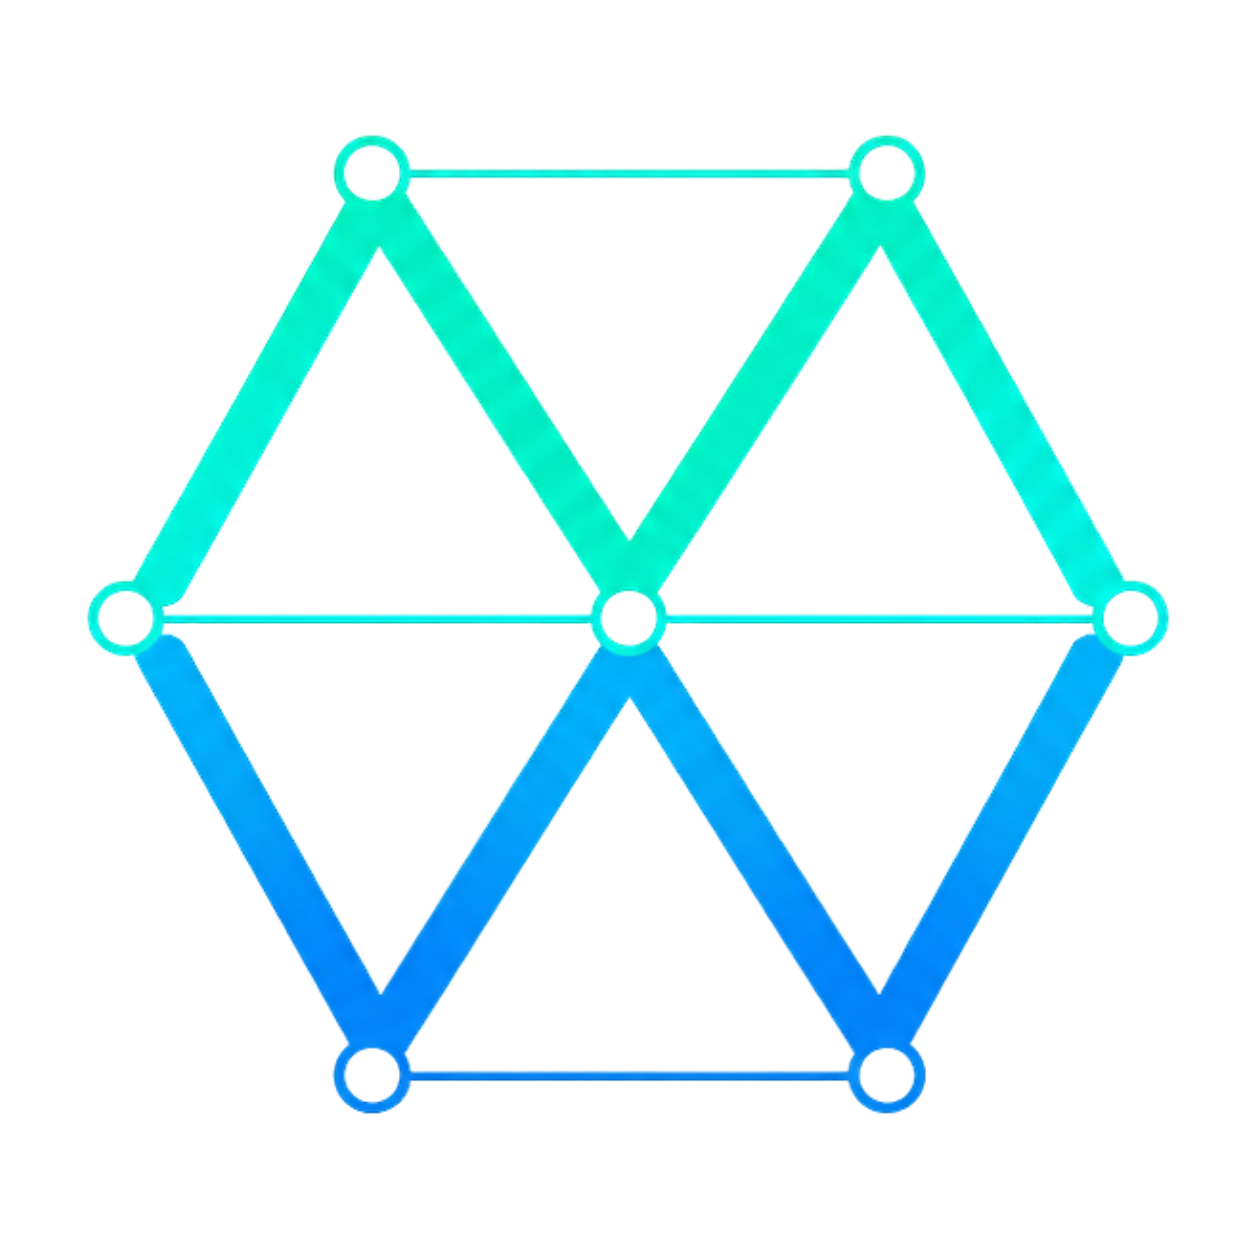
\includegraphics[width=18mm]{mw-logo-mark.png}\\[8pt]
  {\color{white}\Large\bfseries Get started}\\[10pt]
  \color{mwbright}\rule{80mm}{0.4pt}\\[10pt]
  \begin{tabular}{ll}
    \color{mwbright}\textbf{SDK}     & \color{white}\texttt{npm install @meshwhisper/sdk} \\[4pt]
    \color{mwbright}\textbf{Node}    & \color{white}\texttt{docker run meshwhisper/node} \\[4pt]
    \color{mwbright}\textbf{Docs}    & \color{white}\texttt{meshwhisper.org} \\[4pt]
    \color{mwbright}\textbf{Demo}    & \color{white}\texttt{prudence.meshwhisper.org} \\[4pt]
    \color{mwbright}\textbf{Contact} & \color{white}\texttt{anton@gestureloop.com} \\
  \end{tabular}\\[14pt]
  \color{mwbright}\rule{80mm}{0.4pt}\\[8pt]
  {\color{mwlight}\small MIT licensed · Self-hosting always free}
\end{center}
\end{frame}
}

\end{document}
